\documentclass{article}
\usepackage[]{algorithm}
\usepackage[]{algorithmic}
\usepackage{graphicx}

\title{CME211:Final project writeup}
\author{Yunjae Hwang}

\begin{document}
\maketitle

\section*{Introduction}
Many engineering problems can be written linear system of equations
 that is represented as $Ax=b$, where A is a matrix, x and b are vectors.
In this project, the main goal is to implement one of solvers 
(Conjugate-Gradient solver; CG solver) 
that finds the solutions of set of equations.
In order to validate the solver, we employ 2-dimensional heat transfer
 equations described in project instruction part 2.

The problem has isothermal boundaries on the top and bottom wall,
 and periodic boundary conditions for left and right walls.
As the isothermal boundaries have fixed temperatures,
 the implemented program solves for the temperature on the interior nodes.
The following sections describe the programming of the CG solver
 and classes that needed for the heat transfer problem.

\section*{Background on the OOP design}
The C++ codes for setting up and solving the problem are basically 6 cpp files.
Second part of the project requires to implement 2 classes,
 HeatEquation2D and SparseMatrix in heat.cpp and sparse.cpp, respectively.
Short descriptions of each class are :

{\bf HeatEquation2D}
\begin{itemize}
    \item Setup: The methods first read given input file
     and setup up matrix and right hand side vector.
     For convergence of the problem, the signs of elements
      in both matrix and vector switches.
    \item Solve: Calls CGSolver function implemented in CGSolver.cpp
     and the pseudocode is visualized in Algorithm \ref{alg1}.
\end{itemize}

{\bf SparseMatrix}
\begin{itemize}
    \item Resize: Changes the size of the sparse matrix
     by modifying number of row and column.
    \item AddEntry: Add entry of an element, appending row, column
     and element in correspoding data attribute in the class.
    \item ConvertToCSR: Convert COO format sparse matrix to CSR format,
     by calling function "COO2CSR" in COO2CSR.cpp .
    \item MulVec: Multiply the sparse matrix in CSR format to a vector input
\end{itemize}

The steps below are the order of methods running in main.cpp.

\begin{algorithm} 
    \caption{Flow chart of methods implemented in main function}
    \label{alg0}
    \begin{algorithmic}
        \STATE {\bf SparseMatrix::Setup}
        \STATE \qquad Read input file 
        \STATE \qquad Construct $\mathbf{A}$ and $\mathbf{b}$
        \STATE \qquad $\mathbf{A}$
         = -$\mathbf{A}$, $\mathbf{b}$ = -$\mathbf{b}$ (Switch signs)
        \STATE \qquad {\bf A.ConvertToCSR()}

        \STATE {\bf SparseMatrix::Solve}
        \STATE \qquad Call {\bf CGSolver}
    \end{algorithmic}
\end{algorithm}


\section*{CG Solver implementation}
The main task of the first part of the project is
to implement CG algorithm in SparseMatrix::Solve.
The algorithm below(Algorithm \ref{alg1}) summarizes 
the CG algorithm developed in my program.
Basically the same with the description 
in the assignment instruction.
First it has an intial guess of the solution vector 
$\mathbf{u}_0$ with all elements are 100.0
 (which is the average of the $T_c$ and $T_h$).
It computes residual vector $\mathbf{r}_0$ 
and its second norm, accordingly.
After the initilaliztion, while loop starts and interates 
until either the ratio of the two residuals 
becomes less than the tolerance 
($ \|\mathbf{r}_{n+1}\|_2 / \|\mathbf{r}_0\|_2 < \epsilon $) or
the number of iteration exceeds the specified number of iteration 
($n_{iter} > n_{iter,max}$).
Once the while loop finishes, 
the $u_{n+1}$ vector will be returned to main function as the solution $x$.

In addtion to just solving the system, it automatically writes solutions
at the first, last and every 10 iterations.

Implementing "matvecops" significantly reduces the complexity 
in the calculation between a vector and a matrix.
It was used in the first part of the project, but "MulVec" method
 in "SparseMatrix" is used instead.

In addition to this for reducing redundant programming, 
two functions are developed for computing the second norm of a vector 
and inner product of two vectors.

Here is the pseudocode of the algorithm developed in CGSolver.cpp:

\begin{algorithm}[h]
    \caption{Conjugate Gradient (CG) algorithm 
    for solving a linear system: $\mathbf{Ax=b}$}
    \label{alg1}
    \begin{algorithmic}
        \STATE Initialize $\mathbf{u_0}$
        \STATE $\mathbf{r}_0 = \mathbf{b} - \mathbf{A} \mathbf{u}_0$
        \STATE compute $\|\mathbf{r}_0\|_2$
        \STATE $\mathbf{p}_0 = \mathbf{r}_0$
        \PRINT $\mathbf{u}_0$
        \WHILE{$n_{iter} < n_{iter,max}$}
            \STATE $n_{iter} = n_{iter}+1$
            \STATE $\alpha = (\mathbf{r}_n^T \mathbf{r}_n)
                /(\mathbf{p}_n^T \mathbf{A} \mathbf{p}_n)$
            \STATE $\mathbf{u}_{n+1}  
                = \mathbf{u}_n + \alpha_n \mathbf{p}_n$
            \STATE $\mathbf{r}_{n+1}  
                = \mathbf{r}_n + \alpha_n \mathbf{A} \mathbf{p}_n$
            \IF{$ \|\mathbf{r}_{n+1}\|_2 / \|\mathbf{r}_0\|_2 < \epsilon $}
                \STATE \bf{break}
            \ENDIF
            \STATE $\beta_n 
                = (\mathbf{r}_{n+1}^T \mathbf{r}_{n+1})
                /(\mathbf{r}_n^T \mathbf{r}_n)$
            \STATE $\mathbf{p}_{n+1} 
                = \mathbf{r}_{n+1} + \beta_n \mathbf{p}_n $
            \IF{$n_{iter}\% 10 ==0 $}
                \PRINT $\mathbf{u}_n$
            \ENDIF
        \ENDWHILE
        \STATE $\mathbf{x} = \mathbf{u}_{n+1}$
        \PRINT $\mathbf{x}$
    \end{algorithmic}
\end{algorithm}


\section*{Users guide}
This section introduces the way how to compile codes and run them.
The "makefile" automatize compiling and cleaning c++ files efficiently. 
We can do these using following commands:
\begin{verbatim}
make
make clean
\end{verbatim}
Running the first line will compile *.cpp files in the directory,
 link them and ultimately generate the output executable file "main".
The second line is to remove all object(*.o) and editor(~*) files.

The output "main" executable can be ran by typing the command below:
\begin{verbatim}
./main input#.txt solution_prefix
\end{verbatim}
The "input\#.txt"  indicate the input of a heat transfer problem  
and "solution\_prefix" is a prefix of solution output files.
After running the "main" the postprocess can be done by python script.
The python script can be run:
\begin{verbatim}
python3 postprocess.py input#.txt solution_prefix_#.txt
\end{verbatim}
Where input\#.txt is the same input file provided above in the c++ code, 
and solution\#.txt is the output of c++ program.

\section*{Post-processing result}
This section displays results of two input files, input0.txt and input2.txt.
As $T_c=0$ in input0.txt, interior temperature has no variation in length. 
While the result contour in input2.txt shows variation
 in both width and length direction.
\begin{figure}[h!]
\centering
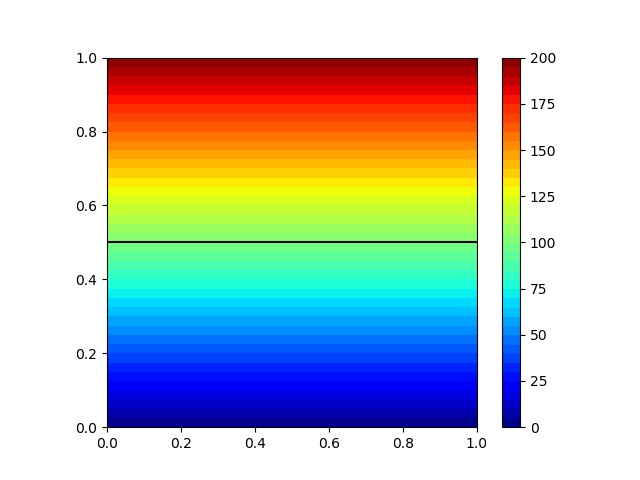
\includegraphics[width=0.48\textwidth]{result0.jpg}
% 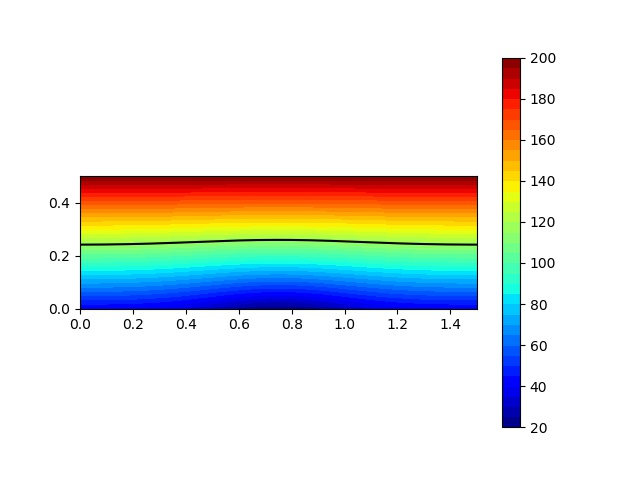
\includegraphics[width=0.80\textwidth]{result1.jpg}
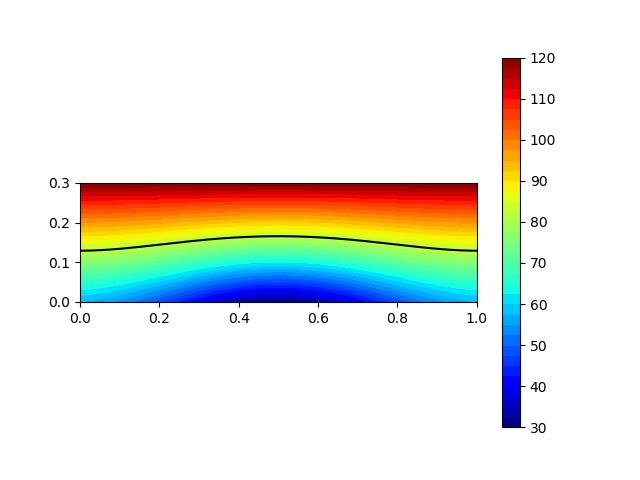
\includegraphics[width=0.48\textwidth]{result2.jpg}
\caption{\label{fig:result} The temperature contours
 in domains of two input files:
input0.txt(left) and input2.txt(right)}
\end{figure}


\section*{Users guide for bonus}
This section is about the bonus of the final project.
Instead of saving the video, it will show the variation of the temperature over iterations.
The way to run the bonus.py is following:

\begin{verbatim}
    python3 bonus.py input#.txt solution_prefix
\end{verbatim}
Where input\#.txt indicates the input file and
 solution\_prefix is the prefix of solution output files.

\begin{thebibliography}{999}
    \bibitem{instruction1}
    \emph{cme211-project-part-1.pdf}. \\
    https://canvas.stanford.edu/courses/87822/files/folder/Final
    \%20Project?preview=3723058

    \bibitem{instruction2}
    \emph{cme211-project-part-2.pdf}. \\
    https://canvas.stanford.edu/courses/87822/files/folder/Final
    \%20Project?preview=3765188

\end{thebibliography}
\end{document}